\documentclass[a4paper, 10pt]{paper}
\usepackage{graphicx}
\usepackage{fullpage}
\usepackage{amsmath}
\usepackage{amssymb}
\usepackage{hyperref}
\usepackage{tcolorbox}
\usepackage{tikz}
%\usepackage{MnSymbol}



\newcommand{\be}{\begin{eqnarray*}}
\newcommand{\ee}{\end{eqnarray*}}
\newcommand{\beq}{\begin{eqnarray}}
\newcommand{\eeq}{\end{eqnarray}}
\newcommand{\bk}{{\mathbf{k}}}
\newcommand{\bK}{{\mathbf{K}}}
\newcommand{\bp}{{\mathbf{p}}}
\newcommand{\bq}{{\mathbf{q}}}
\newcommand{\bm}{{\mathbf{m}}}
\newcommand{\br}{{\mathbf{r}}}
\newcommand{\bu}{{\mathbf{u}}}
\newcommand{\bR}{{\mathbf{R}}}
\newcommand{\bS}{{\mathbf{S}}}
\newcommand{\ba}{{\mathbf{a}}}
\newcommand{\bb}{{\mathbf{b}}}
\newcommand{\bc}{{\mathbf{c}}}
\newcommand{\bd}{{\mathbf{d}}}
\newcommand{\bbe}{{\mathbf{e}}}
\newcommand{\bB}{{\mathbf{B}}}
\newcommand{\bA}{{\mathbf{A}}}
\newcommand{\bE}{{\mathbf{E}}}
\newcommand{\bF}{{\mathbf{F}}}
\newcommand{\bJ}{{\mathbf{J}}}
\newcommand{\bP}{{\mathbf{P}}}
\newcommand{\bX}{{\mathbf{X}}}
\newcommand{\bv}{{\mathbf{v}}}
\newcommand{\bs}{{\mathbf{s}}}
\newcommand{\bfe}{{\mathbf{e}}}
\newcommand{\bt}{{\mathbf{t}}}
\newcommand{\bg}{{\mathbf{g}}}
\newcommand{\dd}{\mathrm{d}}
\newcommand{\bhx}{\hat{\mathbf{x}}}
\newcommand{\bhy}{\hat{\mathbf{y}}}
\newcommand{\bhz}{\hat{\mathbf{z}}}
\newcommand{\bhw}{\hat{\mathbf{w}}}
\newcommand{\bx}{{{\mathbf{x}}}}
\newcommand{\by}{{{\mathbf{y}}}}
\newcommand{\h}{\hat{H}}
\newcommand{\hp}{\hat{P}}
\newcommand{\up}{\uparrow}
\newcommand{\down}{\downarrow}
\newcommand{\ph}{{\phantom{\dagger}}}
\newcommand{\ket}[1]{\left|{#1}\right\rangle}
\newcommand{\bra}[1]{\left\langle{#1}\right|}
\newcommand{\hc}{\mathrm{H.c.}}
\newcommand{\an}[1]{\left(a\right^{#1}}
\newcommand{\ad}[1]{\left(a^\dagger\right^{#1}}
\newcommand{\ado}{a^\dagger}
\newcommand{\bdo}{b^\dagger}
\newcommand{\ddp}{\partial}

\newcommand{\mcA}{\mathcal{A}}
\newcommand{\mcB}{\mathcal{B}}
\newcommand{\mcC}{\mathcal{C}}
\newcommand{\mcD}{\mathcal{D}}
\newcommand{\mcM}{\mathcal{M}}
\newcommand{\mcN}{\mathcal{N}}

%\newcommand{\bn}[1]{\left(b\right^{#1}}
%\newcommand{\bd}[1]{\left(b^\dagger\right^{#1}}

\newcommand{\bn}{\mathbf{n}}
\newcommand{\id}{\mathbb{I}}
\newcommand{\zbb}{\mathbb{Z}}
\newcommand{\zb}{\bar{z}}

\newcommand{\tr}{\mathrm{tr}}
\newcommand{\Tr}{\mathrm{Tr}}

\newcommand{\kb}[2]{\ket{#1}\!\bra{#2}}
\newcommand{\kbd}[2]{\ket{#2}\!\bra{#1}}

\newcommand{\ketx}[1]{\left|{\frac{\partial^{#1}\tilde{u}_n}{\partial {k_x}^{#1}}}\right\rangle}
\newcommand{\brax}[1]{\left\langle{\frac{\partial^{#1}\tilde{u}_n}{\partial {k_x}^{#1}}}\right|}
\newcommand{\kety}[1]{\left|{\frac{\partial^{#1}\tilde{u}_n}{\partial {k_y}^{#1}}}\right\rangle}
\newcommand{\bray}[1]{\left\langle{\frac{\partial^{#1}\tilde{u}_n}{\partial {k_y}^{#1}}}\right|}

\newcommand{\keto}{\ket{\tilde{u}_n}}
\newcommand{\brao}{\bra{\tilde{u}_n}}

\newcommand{\ketxy}[2]{{\left|\frac{\partial^{#1+#2}\tilde{u}_n}{\partial {k_x}^{#1}\partial {k_y}^{#2}}\right\rangle}}
\newcommand{\braxy}[2]{\left\langle{\frac{\partial^{#1+#2}\tilde{u}_n}{\partial {k_x}^{#1}\partial {k_y}^{#2}}}\right|}

\newcommand{\bbn}{\bra{\tilde{n}}}
\newcommand{\bkn}{\ket{\tilde{n}}}
\newcommand{\bbm}{\bra{\tilde{m}}}
\newcommand{\bkm}{\ket{\tilde{m}}}

\newcommand{\kx}{\hat{k}_x}
\newcommand{\ky}{\hat{k}_y}
\newcommand{\xz}{$(x$-$z$}
\newcommand{\yw}{$(y$-$w$}

\begin{document}
\title{EM Response for Quartic Hamiltonian (etc.)---Direct Numerics}
\maketitle
%%%%%%
In this document, we calculate expectation values directly rather than using the nested sums as before, which should be faster and more accurate. 
%%%
\section{Current per Orbital}
We recall that the $2n$ Hamiltonian (in David's notation) is
\be
\h_{2n}&=&\frac{1}{2n}\bigg[\hat{k}_x^{2n}+\hat{k}_y^{2n}\bigg],
\ee
where
\be
\hat{k}_y&=&-\sqrt{\frac{B}{2}}\left(a+a^\dagger\right)\\
\hat{k}_x&=&-i\sqrt{\frac{B}{2}}\left(a-a^\dagger\right).
\ee
To calculate the current per orbital, we require the current operator, which we write as
\be
\hat{I}_y&=&\partial H/\partial k_y.
\ee
Noting that
\be
\partial_{k_y}a=\partial_{k_y}a^\dagger&=&-\frac{1}{\sqrt{2B}}
\ee
we see that
\be
\partial_{k_y}\hat{k}_x&=&0\\
\partial_{k_y}\hat{k}_y&=&1
\ee
(as expected) and so
\be
\partial_{k_y}\h_{2n}&=&\hat{k}_y^{2n-1}.
\ee
The $p$th term in the external potential is 
\be
c_p(2B)^{-p/2}\left(a+a^\dagger\right)^p&=&c_p\frac{(-1)^p}{B^p}\hat{k}_y^{p}.
\ee
Then, the current per orbital expression becomes
\be
\left\langle \hat{I}_y\right\rangle&=&\sum_{\mu\neq\lambda}\bra{\lambda}\hat{I}_y\ket{\mu}\frac{\bra{\mu}\hat{V}(x)\ket{\lambda}}{E_\lambda-E_\mu}+\hc\\
&=&2\sum_{\mu\neq\lambda}\sum_pc_p\frac{(-1)^p}{B^p}\bra{\lambda}\hat{k}_y^{2n-1}\ket{\mu}\frac{\bra{\mu}\hat{k}_y^p\ket{\lambda}}{E_\lambda-E_\mu}.
\ee
For each value of $\lambda,p$, we can calculate these matrix elements and sum over $\mu$ directly. We aim to find the numerical factor that multiplies $c_p$ (setting $B=1$).
%%%
\subsection{Numerical Results}
This is now extremely fast so we calculate up to $n=8$. We plot the results below:
\begin{center}
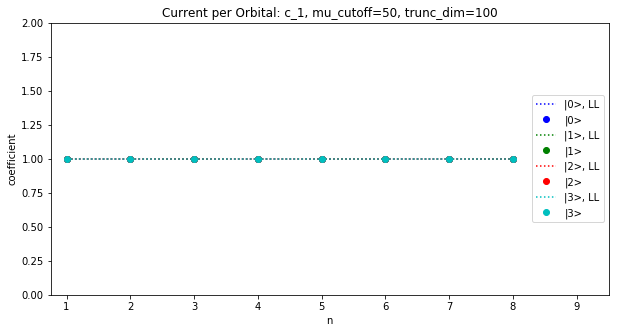
\includegraphics[scale=0.57]{Orbital_c1.png}
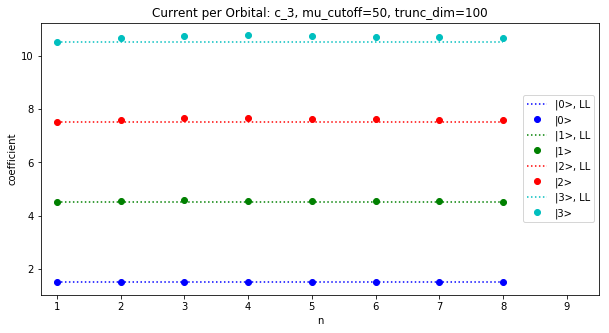
\includegraphics[scale=0.57]{Orbital_c3.png}
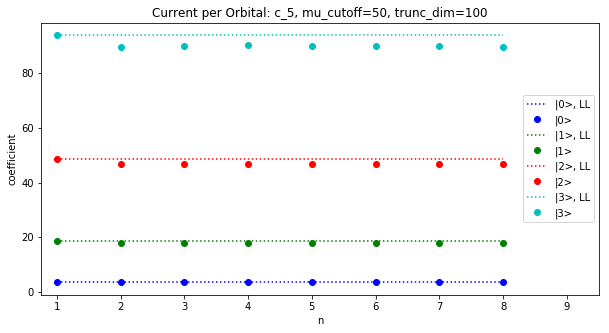
\includegraphics[scale=0.57]{Orbital_c5.png}
\end{center}
These agree with the values calculated using the previous method. The values for $c_1$ are equal to the LL value (topologically protected).
%%%%
%%%%
\section{Current Density}
The current density is given by the expression
\be
\left\langle \hat{J}_y\right\rangle^{2n}_{\lambda}&=&\frac{B}{2\pi}\sum_{r,s}\sum_{\mu\neq\lambda}d_{rs}\bra{\lambda}\hat{I}_y\hat{x}^s\ket{\mu}\frac{\bra{\mu}\hat{x}^r\ket{\lambda}}{E_\lambda-E_\mu}+\hc\\
&=&\frac{B}{2\pi}\sum_{r,p}\sum_{\mu\neq\lambda}d_{r,p-r}\bra{\lambda}\hat{I}_y\hat{x}^{p-r}\ket{\mu}\frac{\bra{\mu}\hat{x}^r\ket{\lambda}}{E_\lambda-E_\mu}
\ee
where we recall that
\be
d_{rs}&=&(-1)^s\left(\begin{array}{c}
r+s\\
s
\end{array}\right)c_{r+s}\\
d_{r,p-r}&=&(-1)^{p-r}\left(\begin{array}{c}
p\\
p-r
\end{array}\right)c_{p}.
\ee
Making the same substitutions as before, this becomes
\be
\left\langle \hat{J}_y\right\rangle^{2n}_{\lambda}&=&\frac{B}{2\pi}2\sum_{\mu\neq\lambda}\sum_{p,r}d_{r,p-r}\frac{(-1)^p}{B^p}\bra{\lambda}\hat{k}_y^{2n-1+p-r}\ket{\mu}\frac{\bra{\mu}\hat{k}_y^r\ket{\lambda}}{E_\lambda-E_\mu}.
\ee
We ignore the factor of $B/2\pi$ (which can be put in by hand later). 
%%%
\subsection{Numerical Results}
\begin{center}
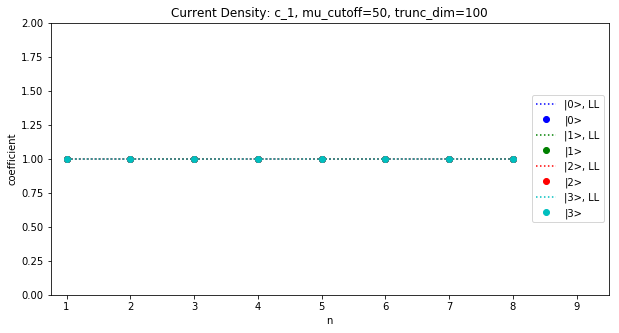
\includegraphics[scale=0.57]{Density_c1.png}
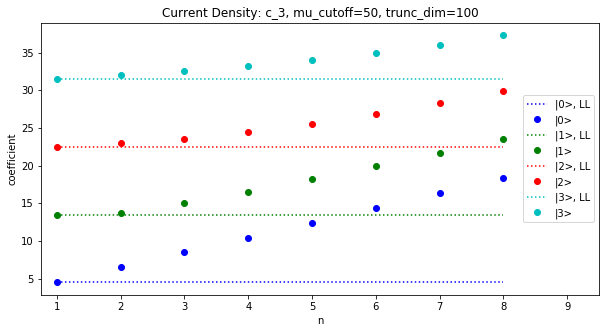
\includegraphics[scale=0.57]{Density_c3.png}
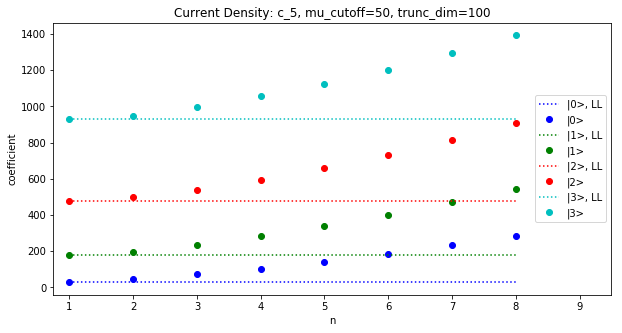
\includegraphics[scale=0.57]{Density_c5.png}
\end{center}
Again, the coefficient of $c_1$ is unchanged (topologically protected), but the others all vary with $n$. The differences from the Landau level case are much larger this time. These values agree with those calculated using the previous method, but the calculation is much faster.




\end{document}